\clearpage
\subsection{Source Code and the Compiler} % (fold)
\label{sub:source_code_and_the_compiler}

The next step in programming language evolution moved from machine level instructions to something more human readable. These languages, known as \textbf{Third Generation Languages}, use move advanced programs than assemblers to convert their instructions into machine code. Programs written in these languages have their code converted to machine code by a \textbf{compiler}.

A \textbf{Compiler} is a program that converts \textbf{Source Code} into machine code that is saved into an executable file called a \emph{Program}. The program can then be executed independent of the compiler and the source code.

Internally, a compiler will perform a number of steps, as shown in \fref{fig:compiler}.

\begin{enumerate}
  \item \textbf{Preprocessing}: The code is read from your source code files. This may involve some processing of the text itself, which includes things like ignoring any comments in the code.
  \item \textbf{Compiling}: The code is then converted into assembly instructions, and an assembly program is output.
  \item \textbf{Assembling}: The assembly version of the program is converted into machine code, and stored in \textbf{object files}.
  \item \textbf{Linking}: In the final step the compiler uses a \textbf{Linker} to join together the machine code from your program, with other machine code you have used from the programming libraries. This then outputs an executable program.
\end{enumerate}

\begin{figure}[h]
   \centering
   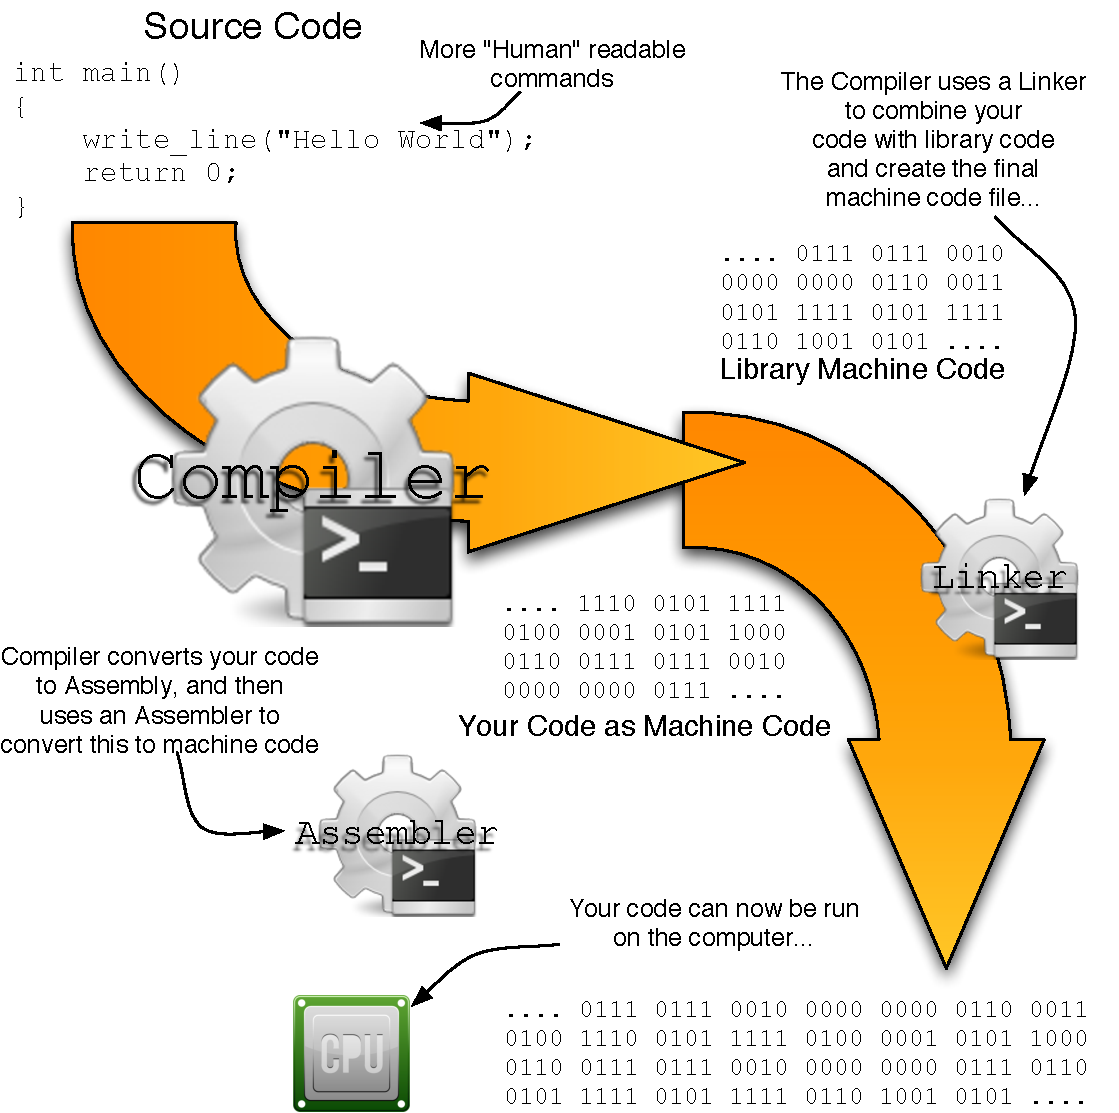
\includegraphics[width=0.7\textwidth]{./topics/programs-and-compilers/diagrams/Compiler} 
   \caption{Compilers turn Source Code into Machine Code}
   \label{fig:compiler}
\end{figure}

\clearpage
\subsubsection{Programming with a Third Generation Language} % (fold)
\label{ssub:programming_with_a_third_generation_language}

\lref{lst:hello-world-c-1} and \lref{lst:hello-world-pas-1} show two examples of source code. This code describes a small program that can be used to output a message to the \nameref{sub:terminal}.

\begin{multicols}{2}
  \ccode{lst:hello-world-c-1}{Example C++ code}{code/c/program-creation/hello-world.c}
  \columnbreak
  \pascode{lst:hello-world-pas-1}{Example Pascal code}{./topics/program-creation/pascal/HelloWorld.pas}
\end{multicols}

The code shown in \lref{lst:hello-world-c-1} shows the code for the C++ program that was used to generate the assembler code, and machine code shown in the previous code listings. This code must be converted by the C++ compiler into machine code before it can be run. It is interesting to note the size of the C++ file: it is only 50 bytes! The compiler converts this 50 bytes into the 13,344 bytes of machine code. 

\lref{lst:hello-world-pas-1} shows the same program written in the Pascal programming language. Like its equivalent C++ code, this must be compiled to create a program you can run.

Programs written in a third generation programming language are much easier to understand than their assembler or machine code counterparts. It is also possible that this code can be compiled to run on different types of CPU, making it more portable. Most modern programming languages are third generation programming languages.


The code that a programmer writes in these languages is called \textbf{Source Code}. Typically source code is saved into a text file with a file extension that helps identify the language it is written in. For example, programs written in the C++ language are saved into files with a {\tt .c} file extension whereas Pascal programs are saved into files with a {\tt .pas} extension.

\mynote{
\begin{itemize}
  \item There are may different Third Generation Languages, including both C++ and Pascal.
  \item Each language has its own compiler that understands that language's code.
  \item The C++ compiler we will use is \textbf{clang++} (or \textbf{g++} - the \textbf{GNU C++ Compiler}).
  \item The Pascal compiler we will use is called \textbf{fpc} - this stands for \textbf{Free Pascal Compiler}.
\end{itemize}
}



% subsubsection programming_with_a_third_generation_language (end)

% subsection source_code_and_the_compiler (end)